\chapter{时空折中算法}
本章主要要介绍时空折中算法的相关理论基础。从最初Martin Hellman的时空折中算法、Ronald Rivest的差异点DP方法到Philippe Oechslin在2003年基于前两种方法提出的彩虹表算法(RainBow Table),时空折中算法已经成为现代密码分析算法中一类极具现实意义的算法之一。这类算法一般都包括了以下两个主要步骤:1,预运算(pre-computation);2,在线分析(online phase)。本章节\ref{sec:3.1},\ref{sec:3.2}和\ref{sec:3.3}将分别介绍Martin Hellman表以及彩虹表的设计原理和构造思想。

我们将在本章中统一使用以下定义:N表示目标密码算法的密钥空间大小;T和M分别表示在线分析的时间代价以及预运算步骤所产生的密钥表空间大小;对于预运算的成功率P,我们通常认为分析者具有足够长的时间,所以该代价一般不作为讨论的内容并且将其粗略等价于穷举所有密钥表空间的时间。
\section{Martin Hellman最初的算法}
\label{sec:3.1}
Martin Hellman在1980年第一次提出基于时间空间折中算法的分组密码算法DES的密码分析\cite{hellman}。攻击者使用的是选择明文攻击,也就是给定一个指定的明文加密后的密文,尝试从密文中分析恢复出这次加密的密钥。因此攻击者所要关心的问题是如何从N中找出对应的密钥,以56比特DES为例,其密钥空间为$N=2^{56}$。(若无特殊说明,下文都将以56比特的DES为目标密码算法)
	\subsection{预运算}
在预运算阶段,算法将首先固定一个目标密文所对应的明文P,一般大小为8个字符(64比特),接着结合P构造如下非逆函数f:
\begin{equation}f(k)=R(S_k(P))
\label{equ:3_1}
\end{equation}
其中P是所选的固定明文信息,S表示伪随机函数,R是一个从密文空间到密文空间的简约(Reduction)函数,并且在下文令S=DES。对于R函数的选择,若无特别说明,我们将假定任一从64比特到56比特的映射函数均可适用。通常为了简便起见,令R函数为仅简单地地去掉64比特的高8位。从而R、S复合而成的f函数可以看作是一个56比特到56比特的伪随机函数。

预运算开始时,算法将选择m个来自密钥空间N的随机密钥作为开始节点(Start Point,简称SP),令其为$SP_1,SP_2,SP_3\ldots SP_{m-1},SP_m$。接着,将$SP_1$作为输入代入公式\eqref{equ:3_1},并迭代t次,得到如下两式\eqref{equ:3_2}和\eqref{equ:3_3}:
\begin{equation}k_i=f(k_{i-1})  (1\leq i \leq t)
\label{equ:3_2}
\end{equation}
\begin{equation}SP_1=k_{10}\xlongrightarrow{f} k_{11}\xlongrightarrow{f} k_{12}\xlongrightarrow{f}\cdots \xlongrightarrow{f} k_{1t}=EP_1
\label{equ:3_3}
\end{equation}

其中,令结束节点(End Point,简称EP)$EP=f(K_{t-1})$。当每个$SP_j$都完成t次迭代后,我们就会得到一张有m对形式如$(SP_j,EP_j) (1\leq j \leq m)$的二元组构成的Hellman表。
\begin{equation}
\underbrace{\begin{bmatrix}
SP_1=k_{10}\xlongrightarrow{f} k_{11}\xlongrightarrow{f} k_{12}\xlongrightarrow{f}\cdots \xlongrightarrow{f} k_{1t}=EP_1 \\
SP_2=k_{20}\xlongrightarrow{f} k_{21}\xlongrightarrow{f} k_{22}\xlongrightarrow{f}\cdots \xlongrightarrow{f} k_{2t}=EP_2 \\
\vdots \\
SP_m=k_{m0}\xlongrightarrow{f} k_{m1}\xlongrightarrow{f} k_{m2}\xlongrightarrow{f}\cdots \xlongrightarrow{f} k_{mt}=EP_m \\
\end{bmatrix}}_{\text{迭代}t\text{次}}
\end{equation}
\begin{equation}
\begin{bmatrix}
SP_1 & EP_1 \\
SP_2 & EP_2 \\
\vdots & \vdots \\
SP_m & EP_m
\end{bmatrix}
\label{equ:3.8}
\end{equation}
这里要注意的是,在SP和EP之间的节点都不会被保存,如\eqref{equ:3.8}式。这些值可以依靠相应的二元组在需要使用的时候可以在线计算生成,这也就是把节省了空间,而关于m,t的选择,就是这个时间于空间折中的选择,一般它们应当满足:
\begin{equation}mt^2=N
\label{equ:3.4}
\end{equation}
而且\eqref{equ:3.4}式也被成为矩阵终止规则(Matrix stopping rule)。根据生日悖论思想,当上式成立时,将不会有太多的重复节点出现,而当m或t过大使得$mt^2>N$,则冲突数量将快速上升,并最后导致Hellman表的成功率下降。而事实上,在实际的密钥攻击过程中,可以允许$mt^2<N$,只不过相应的攻击成功率会有所下降。
	\subsection{在线分析阶段}
        \label{sec:3.1.2}
在线分析阶段,给定已知明文P和对应的密文C,代入R(C)可以得到$y_1$,然后将$y_1$与$EP_i(i=1,2,\ldots ,m)$比较,若存在某个i,使得等式$y_i=EP_i$成立,则会出现以下两种情况:1,加密$y_1$的密钥为$K=k_{i,t-1}$;2,所对应的密钥不在表中,这个现象叫做False alarm。 若等式$y_1=EP_i$不成立,则继续迭代下一步$y_2=f(y_1)$,并重复上一步相同的比较,直到出现以下三种情况:1,找到密钥;2,出现False alarm,就也就假警;3,表搜索结束。简单地讲,在线分析的目的是在Hellman表中搜索出正确的密钥K,使得$K=k_{ij}=y_{t-j}$。需要注意的是,在线分析过程中的$y_j$是可以反复利用与$y_{j+1}$计算的,之后介绍的彩虹表将无法重用。
	\subsection{TMTO曲线}
在介绍TMTO曲线前,我们将先讨论Hellman表的空间代价和时间代价。在忽略二元组$(SP_j,EP_j)$本身大小和一些其他较小的常量后,我们可以计算出存储t张维度为$m	imes t$大小的Hellman表需要的空间M=mt。同时,由于试图要覆盖整个密钥空间,故预运算的代价P=N。在线分析阶段,每一张表的搜索,函数f最多会被调用t次,因此t张表的总时间代价$T=t^2$,由于搜索的代价相对比较低,在这里可以忽略不计。基于上述时间和空间的代价分析就很容易得到TMTO曲线:
\begin{equation}TM^2=N^2\text{并且} P=N
\label{equ:3.5}
\end{equation}
反之,当给定时间代价T和空间代价M时,则可以通过3.5式推出m和t,也就是说可以在时间T和空间M得限制下,从以m,t为参数得Hellman表中找到正确得密钥K。

结合\eqref{equ:3.4}式和\eqref{equ:3.5}式我们得到一个重要的等式:
\begin{equation}T=M=N^{\tfrac{2}{3}}
\label{equ:3.6}
\end{equation}
由等式\eqref{equ:3.6}可知,密码分析者在使用Hellman表来成功破解密钥K所需要的代价会比穷举攻击快$N^{\tfrac{1}{3}}$倍,当然前提都是在基于选择明文的攻击方式下。由伪随机函数S的特性可以得到,只要稍加修改,比如将函数R的输入输出长度改变,我们就能对其他的分组密码算法进行密钥破解。所以,对任意的密钥空间为N的分组密码,利用Hellman算法都能获得以$N^{\tfrac{2}{3}}$为代价的密钥破解成功。而针对其他体制的加密算法的密钥分析,例如以杂凑Hash函数为代表的MD5和SHA-1的加密算法,我们将在下面的彩虹表讨论分析。
	\subsection{密钥分析的成功率}
在上一章\ref{sec:2.4}节密码分析方法的比较中,我们已经得出了相对穷举法百分之百的破解成功率来说,Hellman的时空折中算法并非是100\%能破解成功的,即使你付出了$N^{\tfrac{2}{3}}$的代价。换句话说,也就是这类的时空折中算法是以牺牲少量的成功率为代价换取了在时间或空间上的代价,这也充分体现了折中的这个思想。因此,本节将会重点分析Hellman算法的成功率。其实造成功率损失的根本原因在与算法本身,由于简约函数R仅是从密文空间V到密钥空间N的这么一个映射,而对于两个不同的密文$C_1$,$C_2$,会有一定概率映射到同一个密文,并造成Hellman表中的节点因发生了碰撞而不唯一,如图\ref{fig:3.1}所示,因此导致了最终的破解成功率降低。一般来说,当m,t值越大,节点间发生碰撞合并的概率也就越高。并且由于Hellman表的每个节点都使用相同的R函数,所以一旦表中任意两个节点发生碰撞时,这两个节点之后的所有节点也将会发生碰撞,最坏的情况会导致50\%的效率下降。
\begin{figure}[!ht]
\centering
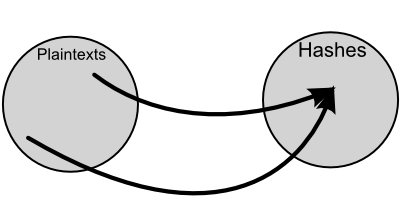
\includegraphics{collision.png}
\caption{碰撞示意图}
\label{fig:3.1}
\end{figure}

成功率是随着m,t的增大非线性地提升。在文献\cite{hellman}中,我们可以得知一张m行,t列的Hellman表能成功破解密钥K的概率公式为:
\begin{equation}
P_{Hellman}\geq \frac{1}{N}\sum_{i=1}^{m}\sum_{j=0}^{t-1}\left(1-\frac{it}{N}\right)^{j+1}
\label{equ:3.7}
\end{equation}
由于有节点的碰撞,单表的破解成功概率会随着表的大小增大而放缓增幅,所以为了得到更高的破解成功概率,我们一般都会使用多张表,例如\eqref{equ:3.4}式中的t张表,并且为了避免表与表之间的链碰撞合并,不同的表当中应当使用不同的函数$R_j(1\leq j \leq t)$使得即使不同表间两个节点相同也难导致链表的合并。因此,我们也就很容易得到了t张Hellman表的总成功率公式:
\begin{equation}
\boxed{P_{Hellman}^{All}\geq 1-\left(1-\frac{1}{N}\sum_{i=1}^{m}\sum_{j=0}^{t-1}\left(1-\frac{it}{N}\right)^{j+1}\right)^t}
\end{equation}
Hellman称上述节点发生碰撞导致链合并的现象为False Alarm,也就是出现了上文\ref{sec:3.1.2}提到的有$y_k=EP_i$,但对应的$k_{i,t-k}$不等于正确密钥。直观上分析,表的规模越大,越有概率发生假警,若假警率过高,则在线分析会花费大量的代价在剔除假警,为此Hellman给出了一个假警上界:
\begin{equation}
E(F)\leq \frac{mt(t+1)}{2N}
\end{equation}
当假警发生时,最坏情况时导致t次函数f的迭代开销,也就是在一开始发生了假警,此时这个代价等同与在线分析时计算$y_1,y_2\ldots y_t$的代价。因此当有$mt^2=N$,且$N\guillemotright 1$时,有$E(F)\leq \frac{1}{2}$,则由于总的开销最多为$\frac{t}{2}$次迭代,从而可以保持假警代价不超过$\frac{t^2}{2}$,即$\frac{T}{2}$。
\section{Ronald Rivest差异点DP方法}
\label{sec:3.2}
在随后的1982年,Ronald Rivest提出了差异点(DP)的概念,通过使用差异点减少对磁盘的访问次数,有效地解决了碰撞的问题,从而降低破解的代价。差异点式满足一套标准的数据点。我们定义密钥的前10比特为一个特定的二进制,为了简便起见,这里设定为零。Rivest提出只存储差异点作为终点,在破解密文时,简单地根据Hellman的方法生成链直到发现一个差异点,当且仅当发现一个差异点时,才在表中进行查找,这可以大大提升算法的性能。

差异点自提出后就被广泛地研究和使用,在1982年和2003年间这一领域的大多数研究都是基于差异点的。Koji Kusuda和Tsutomu Matsumoto\cite{koji}一文中具体讨论了如何提升破解的成功率,通过研究证明调整表中的参数可以降低内存的消耗,以获得更高的成功率,更快地破解密钥。另外,Johan Borst,Bart Preneel和Joos Vandewalle\cite{jbj}共同发表的一篇文献中也对差异点进行了研究,他们介绍了一种分布式的密钥搜索算法,在基于Hellman的假设,认为存储访问代价时微不足道的,研究表明执行分布式密钥搜索时,这个假设不再合理,他们还提出一种可大大减少内存访问次数的折中算法,从而减少与分布式密钥搜索相关的问题。然而,他们的研究在1998年完成,这就意味着他们的工作与2003年Oechslin的工作毫无关联,分布式密钥搜索也与实际的表的生成无关,下面我们将重点介绍Philippe Oechslin在2003年改进后的算法,也就是目前著名的彩虹表算法。
\section{本章小结}
本章主要简要地介绍了2种典型的时空折中算法,Hellman算法和差异点DP算法。时空折中算法主要包括预运算和在线分析两个步骤。Hellman表和彩虹表具有不同的折中曲线,分
别式$TM^2=N^2$和$TM^2=\frac{1}{2}N^2$。重点分析了算法的的成功率,公式的推导演算和证明。
